\chapter{Convolutional Neural Network}
\label{chap:CNN}
Le analisi svolte in questo capitolo seguono la stessa linea del Capitolo \ref{chap:MLP}. Si è voluto dimostrare che andare più in profondità con una CNN non significa migliorare le prestazioni; aggiungere troppi hidden layer porta il modello a non apprendere nulla. Si è dimostrato infine che le residual connection migliorano le cose e mitigano i problemi.

In questo contesto il dataset di riferimento è stato CIFAR-10, già analizzato nella Sezione \ref{sec:CIFAR10}. Il motivo di questa scelta è, data la maggior complessità del dataset in questione, la possibilità di ottenere risultati abbastanza veritieri. MNIST infatti è molto semplice e sbagliare qualcosa e fare male è veramente molto difficile.

\myskip

Le scelte relative a non utilizzare il validation set e a non valutare la loss sul test set sono esattamente le stesse messe in evidenza nel capitolo precedente; è infatti importante ricordare che l'obiettivo non è quello di ottenere alte performance.

Anche in questo caso i nomi degli esperimenti sono relativi al numero di layer del modello analizzato.

%%%%%%%%%%%%%%%%%%%%%%%%%%%%%%%%%%%%%%%%%%%%%%%%%%%%
\section{Analisi senza residual connection}
Se analizziamo inizialmente CNN\_10 e CNN\_13 in Figura \ref{fig:CNNlowdeep}, possiamo osservare l'opposto rispetto ai modelli MLP. Finché il numero di layer non è troppo elevato andare più in profondità migliora sia la loss sul train set che l'accuracy sul test set.

\begin{figure}[htbp]
    \centering
    \begin{subfigure}{0.45\textwidth}
        \centering
        
\includegraphics[width=\textwidth]{immages/4-CNN/loss ok.pdf}
        \caption{Loss}
    \end{subfigure}
    \hfill
    \begin{subfigure}{0.45\textwidth}
        \centering
        
\includegraphics[width=\textwidth]{immages/4-CNN/acc ok.pdf}
        \caption{Accuracy}
    \end{subfigure}
    \caption{Esperimenti CNN non profonde senza residual connection}
    \label{fig:CNNlowdeep}
\end{figure}

Quando però la rete diventa troppo profonda, come per CNN\_30 in Figura \ref{fig:CNNdeepest}, si osserva lo stesso problema dei MLP: il modello non impara niente e la loss rimane molto alta. È chiaro che il problema sia sempre quello del vanishing gradient.

\begin{figure}[htbp]
    \centering
    \begin{subfigure}{0.45\textwidth}
        \centering
        
\includegraphics[width=\textwidth]{immages/4-CNN/loss ko.pdf}
        \caption{Loss}
    \end{subfigure}
    \hfill
    \begin{subfigure}{0.45\textwidth}
        \centering
        
\includegraphics[width=\textwidth]{immages/4-CNN/acc ko.pdf}
        \caption{Accuracy}
    \end{subfigure}
    \caption{Esperimento CNN profonda senza residual connection}
    \label{fig:CNNdeepest}
\end{figure}

%%%%%%%%%%%%%%%%%%%%%%%%%%%%%%%%%%%%%%%%%%%%%%%%%%%%
\section{Analisi con residual connection}
Come nel caso nel MLP anche qua sono state introdotte le residual connection per le varie CNN analizzate precedentemente. Le reti in questione sono esattamente le stesse a cui abbiamo aggiunto i residui tra blocchi convoluzionali.

\myskip

Possiamo osservare contemporaneamente CNN\_res\_16, CNN\_res\_32 e CNN\_res\_56 nella Figura \ref{fig:CNNres}. In questo caso possiamo notare in modo ancora più evidente l'utilità delle residual connection nel mitigare (in questo caso risolvere) il problema del vanishing gradient. I modelli in questione sono tutti confrontabili, sia secondo la loss sul train set sia per l'accuracy sul test set.

\begin{figure}[htbp]
    \centering
    \begin{subfigure}{0.45\textwidth}
        \centering
        
\includegraphics[width=\textwidth]{immages/4-CNN/loss res.pdf}
        \caption{Loss}
    \end{subfigure}
    \hfill
    \begin{subfigure}{0.45\textwidth}
        \centering
        
\includegraphics[width=\textwidth]{immages/4-CNN/acc res.pdf}
        \caption{Accuracy}
    \end{subfigure}
    \caption{Esperimenti CNN con residual connection}
    \label{fig:CNNres}
\end{figure}

\myskip

Come ho fatto nel capitolo precedente ho analizzato i tempi di addestramento per le coppie di reti con e senza residual connection, cioè per CNN\_13 vs CNN\_res\_16 e per CNN\_30 vs CNN\_res\_35. Pensavo che per addestrare una rete con i residui fosse necessario meno tempo, ma il risultato, come mostrato in Figura \ref{fig:CNNtime}, non ha confermato questa mia idea.

\begin{figure}[htbp]
    \centering
    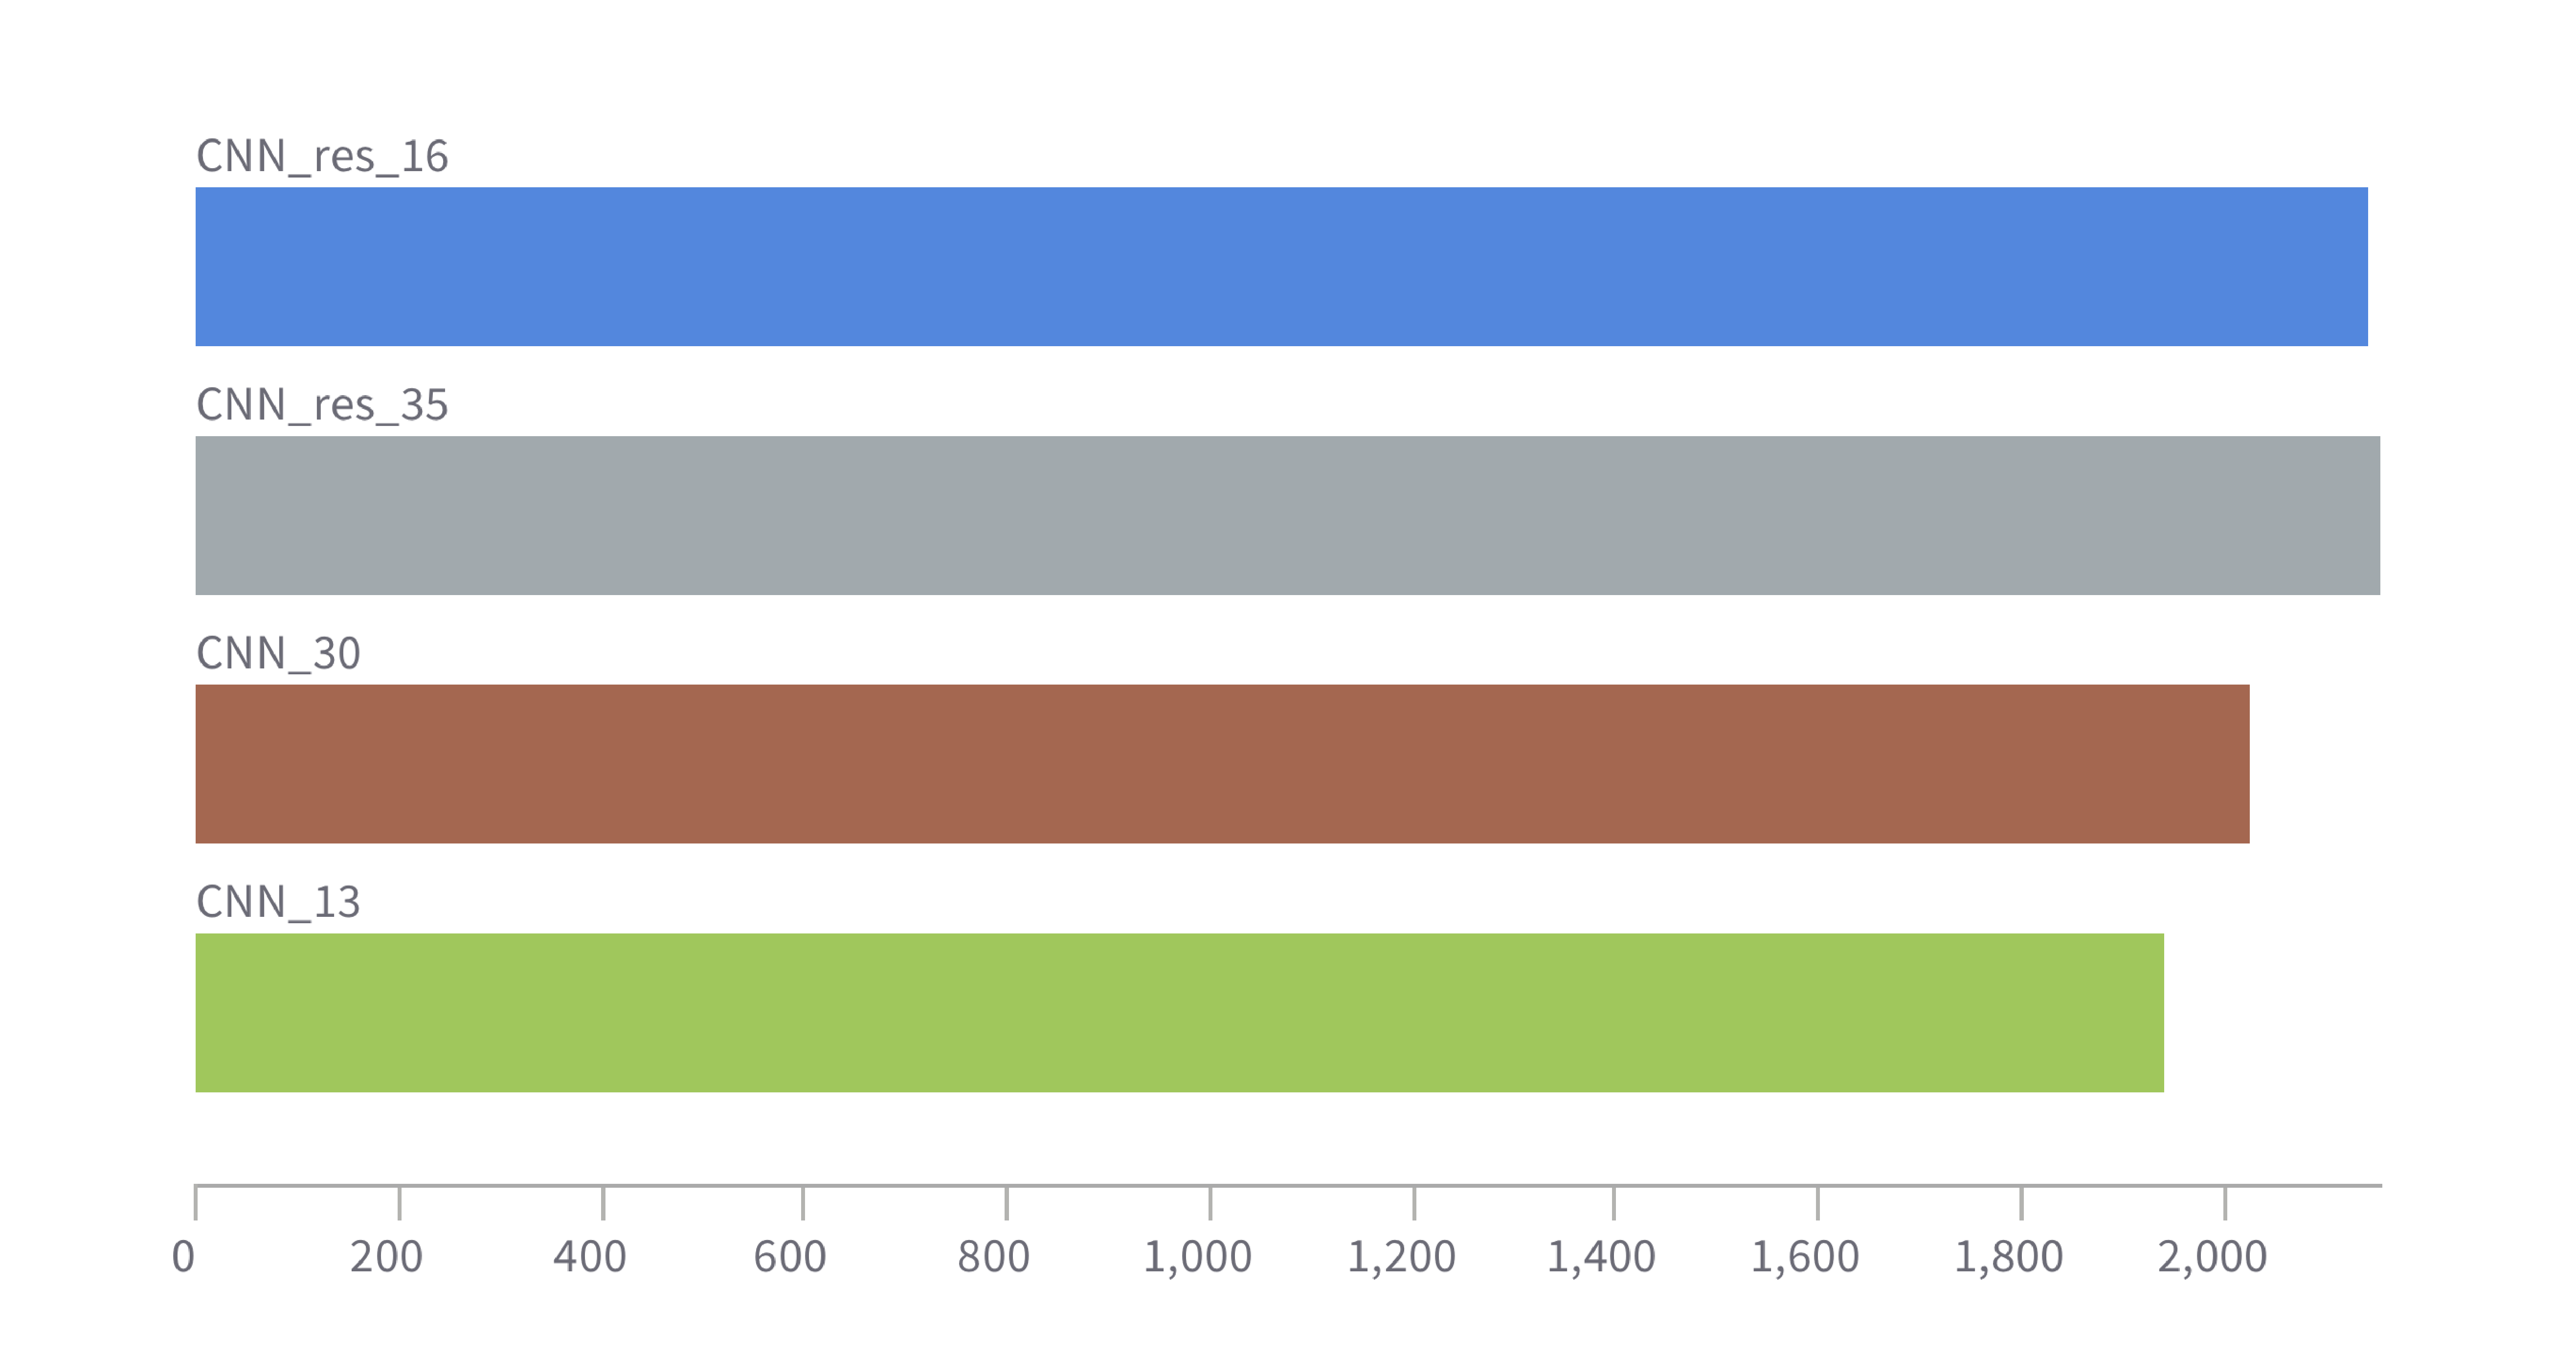
\includegraphics[width=0.6\textwidth]{immages/4-CNN/time.pdf}
    \caption{Training time in CNN}
    \label{fig:CNNtime}
\end{figure}